\begin{activity} \label{A:11.1.1} Let $f(x,y) = 100 - x^2-y^2$ be defined on the rectangular domain $R = [a,b] \times [c,d]$. Partition the interval $[a,b]$ into four uniformly sized subintervals and the interval $[c,d]$ into three evenly sized subintervals as shown in Figure \ref{F:11.1.Domain2}. As we did in Preview Activity \ref{PA:11.1}, we will need a method for identifying the endpoints of each subinterval and the resulting subrectangles.

\begin{figure}[ht]
\begin{center}
  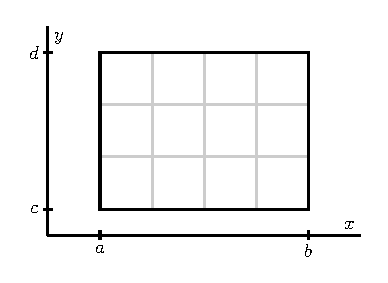
\includegraphics{figures/fig_11_1_rect_general.eps}
\end{center}
\caption{Rectangular domain with subrectangles.}
\label{F:11.1.Domain2}
\end{figure}
 


	\ba
	\item Let $a=x_0 < x_1 < x_2 < x_3 < x_4 =b$ be the endpoints of the subintervals of $[a,b]$ after partitioning. Label these endpoints in Figure \ref{F:11.1.Domain2}.
	
	
	
	\item What is the length $\Delta x$ of each subinterval $[x_{i-1},x_i]$? Your answer should be in terms of $a$ and $b$.
	
	
		
	\item Let $c=y_0 < y_1 < y_2 < y_3 =d$ be the endpoints of the subintervals of $[c,d]$ after partitioning. Label these endpoints in Figure \ref{F:11.1.Domain2}.
	
		
	
	\item What is the length $\Delta y$ of each subinterval $[y_{j-1},y_j]$? Your answer should be in terms of $c$ and $d$.
	
	

	\item The partitions of the intervals $[a,b]$ and $[c,d]$ partition the rectangle $R$ into subrectangles. How many subrectangles are there?
	
	
	
	\item Let $R_{ij}$ denote the subrectangle $[x_{i-1},x_i] \times [y_{j-1},y_j]$. Label each subrectangle in Figure \ref{F:11.1.Domain2}.
	
	
	
	\item What is area $\Delta A$ of each subrectangle?
	
	
	
	\item Now let $[a,b] = [0,8]$ and $[c,d] = [2,6]$.  Let $(x_{11}^*,y_{11}^*)$ be the point in the upper right corner of the subrectangle $R_{11}$. Identify and correctly label this point in Figure \ref{F:11.1.Domain2}. Calculate the product
\[f(x_{11}^*,y_{11}^*) \Delta A.\]
Explain, geometrically, what this product represents.

	
	
	\item For each $i$ and $j$, choose a point $(x_{ij}^*,y_{ij}^*)$ in the subrectangle $R_{i,j}$. Identify and correctly label these points in Figure \ref{F:11.1.Domain2}. Explain what the product
\[f(x_{ij}^*,y_{ij}^*) \Delta A\]
represents.

	
	
	\item \label{p:11.1.Rsum_1} If we were to add all the values $f(x_{ij}^*,y_{ij}^*) \Delta A$ for each $i$ and $j$, what does the resulting number approximate about the surface defined by $f$ on the domain $R$? (You don't actually need to add these values.)

	
	
	\item Write a double sum using summation notation that expresses the arbitrary sum from part ($j$).
	


    \ea


\end{activity}
\begin{smallhint}

\end{smallhint}
\begin{bighint}

\end{bighint}
\begin{activitySolution}
\ba
\item The points $x_0$, $x_1$, $x_2$, $x_3$, and $x_4$ are labeled in the picture below. 
\begin{center}
\setlength{\unitlength}{0.75cm}
\begin{picture}(8.5,6.5)
\put(-0.5,-0.4){$x_0$}
\put(1.7,-0.4){$x_1$}
\put(3.7,-0.4){$x_2$}
\put(5.7,-0.4){$x_3$}
\put(7.7,-0.4){$x_4$}
\put(-1.4,0.05){$y=c$}
%\put(-1.0,1.9){$j=1$}
\put(-1.4,5.9){$y=d$}
\put(0,0){\line(1,0){8}}
\put(0,2){\line(1,0){8}}
\put(0,4){\line(1,0){8}}
\put(0,6){\line(1,0){8}}
\put(0,0){\line(0,1){6}}
\put(2,0){\line(0,1){6}}
\put(4,0){\line(0,1){6}}
\put(6,0){\line(0,1){6}}
\put(8,0){\line(0,1){6}}
\end{picture}
\end{center}

\item The length of the interval $[a,b]$ is $b-a$, and we are dividing the interval into 4 subintervals of equal length. So the length of each subinterval is $\Delta x = \frac{b-a}{4}$. 

\item The points $y_0$, $y_1$, $y_2$, and $y_3$ are labeled in the picture below. 
\begin{center}
\setlength{\unitlength}{0.75cm}
\begin{picture}(8.5,6.5)
\put(-0.5,-0.4){$x_0$}
\put(1.7,-0.4){$x_1$}
\put(3.7,-0.4){$x_2$}
\put(5.7,-0.4){$x_3$}
\put(7.7,-0.4){$x_4$}
\put(-0.7,0){$y_0$}
\put(-0.7,1.9){$y_1$}
\put(-0.7,3.9){$y_2$}
\put(-0.7,5.9){$y_3$}
\put(0,0){\line(1,0){8}}
\put(0,2){\line(1,0){8}}
\put(0,4){\line(1,0){8}}
\put(0,6){\line(1,0){8}}
\put(0,0){\line(0,1){6}}
\put(2,0){\line(0,1){6}}
\put(4,0){\line(0,1){6}}
\put(6,0){\line(0,1){6}}
\put(8,0){\line(0,1){6}}
\end{picture}
\end{center}

\item The length of the interval $[c,d]$ is $d-c$, and we are dividing the interval into 3 subintervals of equal length. So the length of each subinterval is $\Delta y = \frac{d-c}{3}$. 

\item We have 4 subintervals in the $x$ direction and 3 in the $y$ direction, partitioning the rectangle $[a,b] \times [c,d]$ into $3 \times 4 = 12$ subrectangles. 
	
\item As examples, the subrectangle $[x_0,x_1] \times y_0, y_1]$ is $R_{11}$, the lower left subrectangle and the subrectangle $[x_1,x_2] \times y_0, y_1]$ is $R_{21}$, the subrectangle to the right of subrectangle $R_{11}$. The 12 subrectangles are labeled in the figure below.

\begin{center}
\setlength{\unitlength}{0.75cm}
\begin{picture}(8.5,6.5)
\put(-0.5,-0.4){$x_0$}
\put(1.7,-0.4){$x_1$}
\put(3.7,-0.4){$x_2$}
\put(5.7,-0.4){$x_3$}
\put(7.7,-0.4){$x_4$}
\put(-0.7,0){$y_0$}
\put(-0.7,1.9){$y_1$}
\put(-0.7,3.9){$y_2$}
\put(-0.7,5.9){$y_3$}
\put(0.6,0.8){$R_{11}$}
\put(2.6,0.8){$R_{21}$}
\put(4.6,0.8){$R_{31}$}
\put(6.6,0.8){$R_{41}$}
\put(0.6,2.8){$R_{12}$}
\put(2.6,2.8){$R_{22}$}
\put(4.6,2.8){$R_{32}$}
\put(6.6,2.8){$R_{42}$}
\put(6.6,0.8){$R_{41}$}
\put(0.6,4.8){$R_{13}$}
\put(2.6,4.8){$R_{23}$}
\put(4.6,4.8){$R_{33}$}
\put(6.6,4.8){$R_{43}$}
\put(0,0){\line(1,0){8}}
\put(0,2){\line(1,0){8}}
\put(0,4){\line(1,0){8}}
\put(0,6){\line(1,0){8}}
\put(0,0){\line(0,1){6}}
\put(2,0){\line(0,1){6}}
\put(4,0){\line(0,1){6}}
\put(6,0){\line(0,1){6}}
\put(8,0){\line(0,1){6}}
\end{picture}
\end{center}
	
\item Since each subrectangle has side lengths $\frac{b-a}{4}$ and $\frac{d-c}{3}$, the area $\Delta A$ of each subrectangle is $\Delta A = \left(\frac{b-a}{4}\right) \left(\frac{d-c}{3}\right)$. 
	
	
\item With $[a,b] = [0,8]$ and $[c,d] = [2,6]$, we have $\Delta x = 2$ and $\Delta y = \frac{4}{3}$. So $(x_{11}^*,y_{11}^*) 0 \left(2, \frac{4}{3}\right)$ as shown in the figure below. Then
\[f(x_{11}^*,y_{11}^*) \Delta A = f\left(2, \frac{4}{3}\right) (2)\left(\frac{4}{3}\right) = \left(\frac{848}{9}\right)\frac{8}{3} = \frac{6784}{27} \approx 251.26.\]
This result represents the volume of a box with height $f(x_{11}^*,y_{11}^*)$ and base given be the rectangle $[x_0, x_1] \times [y_0, y_1]$. 

\begin{center}
\setlength{\unitlength}{0.75cm}
\begin{picture}(8.5,6.5)
\put(-0.5,-0.4){$x_0$}
\put(1.7,-0.4){$x_1$}
\put(3.7,-0.4){$x_2$}
\put(5.7,-0.4){$x_3$}
\put(7.7,-0.4){$x_4$}
\put(-0.7,0){$y_0$}
\put(-0.7,1.9){$y_1$}
\put(-0.7,3.9){$y_2$}
\put(-0.7,5.9){$y_3$}
\put(0.6,0.8){$R_{11}$}
\put(2.6,0.8){$R_{21}$}
\put(4.6,0.8){$R_{31}$}
\put(6.6,0.8){$R_{41}$}
\put(0.6,2.8){$R_{12}$}
\put(2.6,2.8){$R_{22}$}
\put(4.6,2.8){$R_{32}$}
\put(6.6,2.8){$R_{42}$}
\put(6.6,0.8){$R_{41}$}
\put(0.6,4.8){$R_{13}$}
\put(2.6,4.8){$R_{23}$}
\put(4.6,4.8){$R_{33}$}
\put(6.6,4.8){$R_{43}$}
\put(2,2){\circle*{0.15}}
\put(2.05,2.15){\scriptsize{$(x_{11}^*,y_{11}^*)$}}
\put(0,0){\line(1,0){8}}
\put(0,2){\line(1,0){8}}
\put(0,4){\line(1,0){8}}
\put(0,6){\line(1,0){8}}
\put(0,0){\line(0,1){6}}
\put(2,0){\line(0,1){6}}
\put(4,0){\line(0,1){6}}
\put(6,0){\line(0,1){6}}
\put(8,0){\line(0,1){6}}
\end{picture}
\end{center}
	
	
	\item For each $i$ and $j$, let $(x_{ij}^*,y_{ij}^*)$ be the upper right corner of the subrectangle $R_{i,j}$. These points are marked and labeled in the figure below. 
Identify and correctly label these points in Figure \ref{F:11.1.Domain2}. Explain what the product
\[f(x_{ij}^*,y_{ij}^*) \Delta A\]
represents.

\begin{center}
\setlength{\unitlength}{0.75cm}
\begin{picture}(8.5,6.5)
\put(-0.5,-0.4){$x_0$}
\put(1.7,-0.4){$x_1$}
\put(3.7,-0.4){$x_2$}
\put(5.7,-0.4){$x_3$}
\put(7.7,-0.4){$x_4$}
\put(-0.7,0){$y_0$}
\put(-0.7,1.9){$y_1$}
\put(-0.7,3.9){$y_2$}
\put(-0.7,5.9){$y_3$}
\put(0.6,0.8){$R_{11}$}
\put(2.6,0.8){$R_{21}$}
\put(4.6,0.8){$R_{31}$}
\put(6.6,0.8){$R_{41}$}
\put(0.6,2.8){$R_{12}$}
\put(2.6,2.8){$R_{22}$}
\put(4.6,2.8){$R_{32}$}
\put(6.6,2.8){$R_{42}$}
\put(6.6,0.8){$R_{41}$}
\put(0.6,4.8){$R_{13}$}
\put(2.6,4.8){$R_{23}$}
\put(4.6,4.8){$R_{33}$}
\put(6.6,4.8){$R_{43}$}
\put(2,2){\circle*{0.15}}
\put(2,4){\circle*{0.15}}
\put(2,6){\circle*{0.15}}
\put(4,2){\circle*{0.15}}
\put(4,4){\circle*{0.15}}
\put(4,6){\circle*{0.15}}
\put(6,2){\circle*{0.15}}
\put(6,4){\circle*{0.15}}
\put(6,6){\circle*{0.15}}
\put(8,2){\circle*{0.15}}
\put(8,4){\circle*{0.15}}
\put(8,6){\circle*{0.15}}
\put(2.05,2.15){\scriptsize{$(x_{11}^*,y_{11}^*)$}}
\put(2.05,4.15){\scriptsize{$(x_{12}^*,y_{12}^*)$}}
\put(2.05,6.15){\scriptsize{$(x_{13}^*,y_{13}^*)$}}
\put(4.05,2.15){\scriptsize{$(x_{21}^*,y_{21}^*)$}}
\put(4.05,4.15){\scriptsize{$(x_{22}^*,y_{22}^*)$}}
\put(4.05,6.15){\scriptsize{$(x_{23}^*,y_{23}^*)$}}
\put(6.05,2.15){\scriptsize{$(x_{31}^*,y_{31}^*)$}}
\put(6.05,4.15){\scriptsize{$(x_{32}^*,y_{32}^*)$}}
\put(6.05,6.15){\scriptsize{$(x_{33}^*,y_{33}^*)$}}
\put(8.05,2.15){\scriptsize{$(x_{41}^*,y_{41}^*)$}}
\put(8.05,4.15){\scriptsize{$(x_{42}^*,y_{42}^*)$}}
\put(8.05,6.15){\scriptsize{$(x_{43}^*,y_{43}^*)$}}
\put(0,0){\line(1,0){8}}
\put(0,2){\line(1,0){8}}
\put(0,4){\line(1,0){8}}
\put(0,6){\line(1,0){8}}
\put(0,0){\line(0,1){6}}
\put(2,0){\line(0,1){6}}
\put(4,0){\line(0,1){6}}
\put(6,0){\line(0,1){6}}
\put(8,0){\line(0,1){6}}
\end{picture}
\end{center}
	
	
\item If we add all the values $f(x_{ij}^*,y_{ij}^*) \Delta A$ for each $i$ and $j$, the resulting number approximates the volume of the solid bounded above by the surface defined by $f$ and below by the rectangle $R$. 

	
	
\item A double sum that expresses the arbitrary sum from part ($j$) is
\[\sum_{j=1}^3 \sum_{i=1}^4 f(x_{ij}^*,y_{ij}^*) \Delta A.\]
	


\ea

\end{activitySolution}
\aftera
